\chapter{Resultados Obtidos}
\label{cap:impl}

Para realização dos testes, foram
selecionados 6 tópicos distribuídos em duas categorias diferentes, que são:
Comentários políticos e Comentários sobre filmes. Foram escolhidas duas
categorias distintas com o objetivo de avaliar a assertividade do método
desenvolvido em diferentes assuntos e contextos.

\section{Comentários Políticos}

De forma a realizar testes sobre um contexto de comentários políticos, foi
executado o método de Propagação Dupla, através dos próprios comentários e então
selecionada a palavra \textit{``Trump''}, como a palavra alvo para
restrição na análise de comentários. Desta forma, os tópicos selecionados para
essa análise foram:

\begin{itemize}
  \item
  \textit{Donald Trump to strip all funding from State Dept team promoting
  women's rights around the world - Leaked plan comes as First Daughter Ivanka
  defends her father's record with women}: esse tópico contém 9246
  comentários e encontra-se disponível em
  \textit{\url{https://www.reddit.com/r/worldnews/comments/67ivae/donald_trump_to_strip_all_funding_from_state_dept/}}
  e refere-se a decisão do presidente dos Estados Unidos da América, Donald
  Trump, em remover fundos de promoção ao direito das mulheres.  
  \item
  \textit{Sweden asks the U.S. to explain Trump comment on
  Sweden}: esse tópico contém 10927
  comentários e encontra-se disponível em
  \textit{\url{https://www.reddit.com/r/worldnews/comments/5uzetf/sweden_asks_the_us_to_explain_trump_comment_on/}}
  e se refere aos comentários feitos do presidente dos Estados Unidos da
  América, Donald Trump, sobre a Suécia.
  
  \item\textit{“Canada will welcome you,” Trudeau invites refugees as Trump bans
  them}: esse tópico contém 9113
  comentários e encontra-se disponível em
  \textit{\url{https://www.reddit.com/r/worldnews/comments/5qqa51/canada_will_welcome_you_trudeau_invites_refugees/}}
  e refere-se a declaração do primeiro ministro canadense sobre decisão de
  receber refugiados. Neste declaração, o primeiro ministro canadense afirma que
  os refugiados serão bem-vindos no Canadá.
\end{itemize}

Através da aplicação do método desenvolvido nos tópicos citados anteriormente,
foram obtidos os seguintes resultados com relação a assertividade:

\begin{figure}[!htbp]
\centering
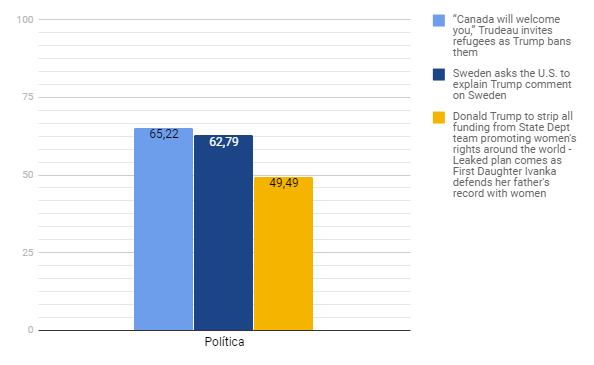
\includegraphics[height=300px]{imagens/politica1.png}
\caption{Assertividade da ferramenta desenvolvida com relação a comentários de
política.}
\label{fig:pol1}
\end{figure}

A fim de se determinar se os diferentes resultados obtidos por Hutto
\cite{conf/icwsm/HuttoG14} sobre a análise de \textit{tweets}, avaliações
de produtos da Amazon e editoriais do New York Times, foram resultados pela
diferença de contexto ou por seus corpos conterem diferentes tamanhos, foi
também conduzida uma análise separando todos os comentários de política em três
categorias, comentários com 144 caracteres ou menos, similares a
\textit{``tweets''}, tópicos com menos de 1000 caracteres e tópicos com 1000
caracteres ou mais. 

\newpage 
A partir dessa análise foram obtidos os seguintes
resultados:

\begin{figure}[!htbp]
\centering
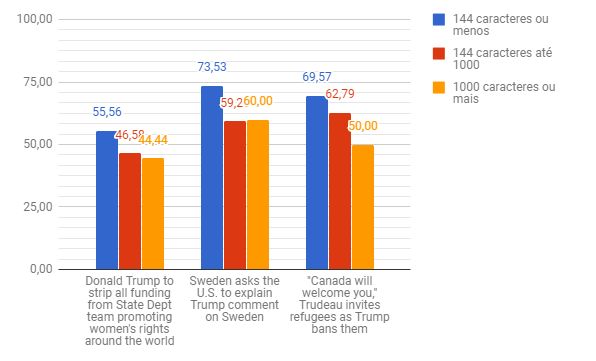
\includegraphics[height=300px]{imagens/politica2.png}
\caption{Assertividade da ferramenta desenvolvida com relação a comentários de
política por tamanho.}
\label{fig:pol2}
\end{figure}


\section{Comentários sobre Filmes}

De forma a executar as mesmas análises realizadas sobre comentários políticos,
foi selecionada a palavra \textit{``movie''}, como uma palavra alvo de restrição
na análise de comentários, em conjunto com o método de Propagação Dupla executado
sobre os próprios comentários. Desta forma, os tópicos selecionados para
essa análise foram:

\begin{itemize}
  \item
  \textit{Official Discussion - mother! [SPOILERS]}: esse tópico contém 5297
  comentários e encontra-se disponível em
  \textit{\url{https://www.reddit.com/r/movies/comments/706y1p/official_discussion_mother_spoilers/}}
  e apresenta a avaliação do filme \textit{``Mother!''}.
  \item
  \textit{Official Discussion: Gerald's Game [SPOILERS]}: esse tópico contém 892
  comentários e
  encontra-se disponível em
  \textit{\url{https://www.reddit.com/r/movies/comments/73g2fx/official_discussion_geralds_game_spoilers/}}
  e apresenta a avaliação do filme \textit{``Gerald's Game''}.
    \item
  \textit{Official Discussion: The Mummy (2017) [SPOILERS]}: esse tópico contém
  1333 comentários e
  encontra-se disponível em
  \textit{\url{https://www.reddit.com/r/movies/comments/6g5lmo/official_discussion_the_mummy_2017_spoilers/}}
  e apresenta a avaliação do filme \textit{``The Mummy''}.
  
\end{itemize}


Através da aplicação do método desenvolvido nos tópicos citados anteriormente,
foram obtidos os seguintes resultados com relação a assertividade:

\begin{figure}[!htbp]
\centering
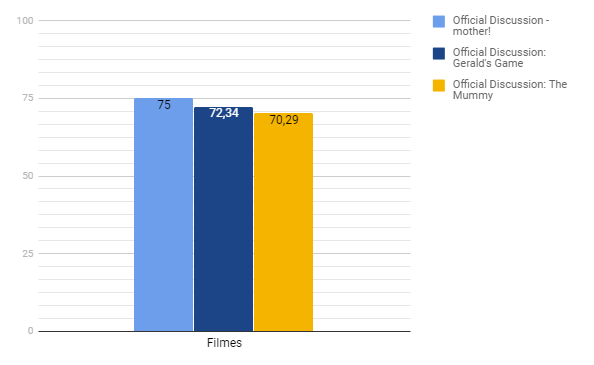
\includegraphics[height=300px]{imagens/filmes1.png}
\caption{Assertividade da ferramenta desenvolvida com relação a comentários de
filmes.}
\label{fig:fil1}
\end{figure}


Também, com o objetivo de demonstrar a assertividade da ferramenta com relação a
quantidade de caracteres por comentário, foi conduzida uma análise separando
todos os comentários de filmes em três categorias de forma a espelhar o
realizado com tópicos de política. Comentários com 144 caracteres ou menos,
similares a \textit{``tweets''}, tópicos com menos de 1000 caracteres e tópicos com 1000 caracteres ou mais. 

\newpage 
A partir dessa análise foram obtidos os seguintes
resultados:

\begin{figure}[!htbp]
\centering
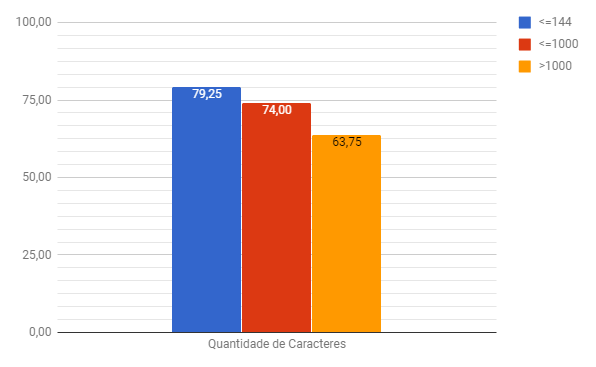
\includegraphics[height=300px]{imagens/filmes2.png}
\caption{Assertividade da ferramenta desenvolvida com relação a comentários de
filmes por tamanho.}
\label{fig:fil2}
\end{figure}

\section{Análise dos Resultados Obtidos}

Através dos resultados
apresentados anteriormente, pode-se verificar que a ferramenta apresentou maior
assertividade ao análisar comentários de filmes (Figura \ref{fig:fil1}) do
que comentários políticos (Figura \ref{fig:pol1}).
Neste contexto, o resultado se mostrou similar ao apresentado por Pålsson e
Szerszen de 72,3\% \cite{SentimentinSocialMedia}.

Já com relação aos tópicos relacionados a política, a ferramenta
apresentou uma baixa assertividade, chegando a apresentar assertividade similar
a uma classificação realizada de forma aleatória, o que naturalmente iria
classificar os comentários com 50\% de acerto eventualmente.

Destaca-se que os tópicos de discussão de filmes encorajam o leitor a avaliar o
filme que está sendo discutido apresentando uma enquete em seu corpo, enquanto
os comentários sobre política apresentam no conteúdo de seu tópico somente um
\textit{link} direto para a notícia original. 

Como o \ac{VADER} faz uso de um
dicionário para a avaliação dos sentimentos, e nos tópicos relacionados com
política não é pedido que o autor do comentário expresse sua opinião sobre o
que estamos querendo avaliar, o \ac{VADER} acaba atribuindo sentimentos não
existentes ou com sua polaridade errada em determinadas frases, como por
exemplo: 

\textit{``\ldots What if he is just like trump and trump's useless
father\ldots``}. 

Neste caso, o dicionário irá avaliar de forma positiva o
comentário pois a palavra \textit{``like''}, quando utilizada com o significado
de ``gostar'' apresenta um sentimento positivo, porém, a palavra
\textit{``like''} neste caso está sendo utilizada como comparação, fazendo com
que a ferramenta apresente o sentimento errado.

Com relação a análise referente a quantidade de caracteres, apresentadas através
das Figuras \ref{fig:pol2} e \ref{fig:fil2}, pode-se verificar que a ferramenta
demonstra a tendência de perder a sua assertividade conforme o número de
caracteres análisados, pois tanto no contexto de comentários de filmes, quanto
no contexto de comentários políticos, a ferramenta apresentou perda na
assertividade conforme os comentários ficaram mais extensos.
